\documentclass[aspectratio=169,11pt]{beamer}
\usepackage[T1]{fontenc}
\usepackage[utf8]{inputenc}
\usepackage{lmodern}
\usetheme{buet}

\title[CaPT \;$\cdot$\; NeurIPS 2025]
      {All You Need is One:\\Capsule Prompt Tuning with a Single Vector}
\author[Quazi Samiha Tasnim \;\&\; Fawzia Fairooz]{Quazi Samiha Tasnim \and Fawzia Fairooz}
\date{\today}
\footmiddle{All You Need is One: Capsule Prompt Tuning with a Single Vector}

\hypersetup{pdftitle={All You Need is One: Capsule Prompt Tuning with a Single Vector},
            pdfauthor={Quazi Samiha Tasnim, Fawzia Fairooz}}

\begin{document}

% =====================================================================
\begin{frame}[plain]
\begin{tikzpicture}[remember picture,overlay]
  \fill[navy] (current page.north west) rectangle ([yshift=-3.5cm]current page.north east);
  \fill[accent] ([yshift=-3.5cm]current page.north west) rectangle ([yshift=-3.58cm]current page.north east);
  \node[anchor=north west] (logo) at ([xshift=0.5cm,yshift=-0.3cm]current page.north west)
       {
\includegraphics[height=1.0cm]{figures/buet_logo.png}};
  \node[anchor=west, text=white, font=\footnotesize, align=left] at ([xshift=0.15cm]logo.east)
       {Bangladesh University of Engineering and Technology (BUET)\\Department of Computer Science and Engineering};
  \node[text=white, font=\LARGE\bfseries, align=center] at ([yshift=-2.3cm]current page.north)
       {All You Need is One:\\[2pt] Capsule Prompt Tuning with a Single Vector};
  \node[text=navy, font=\normalsize\bfseries, align=center] at ([yshift=-3.95cm]current page.north)
       {CSE 6709: Deep Learning};
  \node[text=softgray, font=\footnotesize, align=center] at ([yshift=-4.4cm]current page.north)
       {Paper Presentation \;$\cdot$\; Liu \textit{et al.}, NeurIPS 2025};

  \node[anchor=north, align=center, font=\small] at ([xshift=-4.9cm,yshift=-4.95cm]current page.north)
       {{\color{accent}\bfseries Presented To}\\[3pt]
        \textbf{Dr. Mahmuda Naznin}\\ Professor\\ CSE Dept, BUET};
  \node[anchor=north, align=center, font=\small] at ([xshift=0cm,yshift=-4.95cm]current page.north)
       {{\color{accent}\bfseries Presented By}\\[3pt]
        \textbf{Quazi Samiha Tasnim}\\ ID: 0424052086\\ MSc Engg., CSE Dept, BUET};
  \node[anchor=north, align=center, font=\small] at ([xshift=4.9cm,yshift=-4.95cm]current page.north)
       {{\color{accent}\bfseries Presented By}\\[3pt]
        \textbf{Fawzia Fairooz}\\ ID: 0423052028\\ MSc Engg., CSE Dept, BUET};
  \node[font=\footnotesize, text=softgray] at ([yshift=0.45cm]current page.south) {\insertdate};
\end{tikzpicture}
\end{frame}

% =====================================================================
\begin{frame}{Outline}
\begin{columns}[T]
\column{0.45\textwidth}
\begin{enumerate}
  \item Introduction
  \begin{itemize}
    \item \footnotesize About the Paper
    \item \footnotesize Background
  \end{itemize}
  \item Challenges
  \item Motivation
  \item Related Work
  \item Methodology
  \item Experiments \& Results
\end{enumerate}
\column{0.45\textwidth}
\begin{enumerate}\setcounter{enumi}{6}
  \item Contributions
  \item Limitations (Research Gaps)
  \item Our Proposal
  \item Conclusion
\end{enumerate}
\end{columns}
\end{frame}

% =====================================================================
\section{Introduction}

\begin{frame}{Introduction}
\begin{columns}[c]
\column{0.60\textwidth}
\small What does the title mean?\par\vspace{6pt}
\begin{tikzpicture}[
    key/.style={rounded corners=3pt, line width=0.8pt, minimum width=2.7cm, minimum height=0.9cm,
                align=center, font=\small\bfseries},
    txt/.style={text width=4.6cm, align=left, font=\small, anchor=west}]
  \node[key, draw=accent, fill=accent!8, text=accent] (k1) at (0,0)    {All You Need\\is One};
  \node[txt] at (1.6,0)    {Just \textbf{one} small vector per layer is enough.};
  \node[key, draw=navy, fill=navylight, text=navy] (k2) at (0,-1.3)  {Capsule};
  \node[txt] at (1.6,-1.3) {A tiny package of two things: \textbf{the task} and \textbf{the input}.};
  \node[key, draw=good, fill=good!8, text=good] (k3) at (0,-2.6)     {Prompt Tuning};
  \node[txt] at (1.6,-2.6) {Keep the LLM frozen; learn only a few \textbf{prompt} vectors.};
\end{tikzpicture}

\vspace{8pt}
\small The paper proposes \textbf{CaPT}, a simple prompt-tuning method that uses a
\textbf{single capsule prompt} instead of many soft prompts.
\column{0.36\textwidth}
\begin{block}{Paper Info}
\footnotesize
\textbf{Title:} All You Need is One: Capsule Prompt Tuning with a Single Vector\\[4pt]
\textbf{Authors:} Yiyang Liu, \dots, Qifan Wang, Cheng Han\\[4pt]
\textbf{Venue:} NeurIPS 2025\\[4pt]
\textbf{Area:} Parameter-efficient fine-tuning (PEFT) of LLMs\\[4pt]
\textbf{Code:} \href{https://github.com/comeandcode/CaPT}{\textcolor{navymid}{\underline{\texttt{github.com/comeandcode/CaPT}}}}
\end{block}
\end{columns}
\end{frame}

\begin{frame}{Background: Adapting a Large Language Model}
\begin{columns}[c]
\column{0.42\textwidth}
\begin{itemize}\setlength\itemsep{5pt}
  \item \textbf{Full fine-tuning} updates \emph{all} weights $\Rightarrow$ costly for every new task.
  \item \textbf{PEFT} freezes the model and trains a \emph{tiny} part.
  \item \textbf{Prompt tuning} (a PEFT family): learn a few vectors (\emph{soft prompts}) and put them in front of the input.
  \item \textbf{Deep prompt tuning} (P-Tuning v2): new prompts at \emph{every} layer.
\end{itemize}
\column{0.54\textwidth}
\centering
\begin{tikzpicture}[x=6.2mm]
  \foreach \i in {0,1,2} \node[ptok] at (\i,0) {$P$};
  \foreach \i/\t in {4/$x_1$,5/$x_2$,6/$x_3$,7/$\cdots$,8/$x_n$} \node[tok] at (\i,0) {\t};
  \draw[decorate,decoration={brace,mirror,amplitude=4pt}] (-0.4,-0.4) -- (2.4,-0.4)
        node[midway,below=4pt,font=\scriptsize,text=accent] {trainable soft prompts};
  \draw[decorate,decoration={brace,mirror,amplitude=4pt}] (3.6,-0.4) -- (8.4,-0.4)
        node[midway,below=4pt,font=\scriptsize] {input tokens};
  \node[box, minimum width=5.6cm, minimum height=1.0cm] (llm) at (4,1.6)
        {\textbf{Pre-trained LLM}\\(frozen)};
  \draw[arr] (4,0.35) -- (llm.south);
  \node[boxgray, minimum width=2cm] (out) at (4,3.0) {Output};
  \draw[arr] (llm.north) -- (out.south);
\end{tikzpicture}
\end{columns}
\end{frame}

% =====================================================================
\section{Challenges}

\begin{frame}{Challenges of Soft Prompts}
\small Despite their success, current soft prompt-based methods have \textbf{two main limitations}:
\begin{columns}[T]
\column{0.48\textwidth}
\begin{itemize}
  \item \hl{I. Limited Capability}
  \begin{itemize}\footnotesize\setlength\itemsep{1pt}
    \item Learn only \textbf{task-aware} guidance, the same for every input.
    \item Mostly \textbf{attend to each other}, barely to key input tokens.
    \item So they adapt poorly to \textbf{different inputs}.
  \end{itemize}
\end{itemize}
\column{0.48\textwidth}
\begin{itemize}
  \item \hl{II. Inefficient Searching}
  \begin{itemize}\footnotesize\setlength\itemsep{1pt}
    \item Best prompt length needs a slow \textbf{grid search}.
    \item Ends with \textbf{many prompts} $\Rightarrow$ longer input, more training cost.
    \item Searched prompts may still miss the task; some even \textbf{hurt} accuracy.
  \end{itemize}
\end{itemize}
\end{columns}
\vspace{6pt}
\begin{block}{Root cause}
Task-aware prompts \textbf{lack instance-aware information} $\Rightarrow$ weak attention with the input.
\end{block}
\end{frame}

% =====================================================================
\section{Motivation}

\begin{frame}{Motivation of the Paper}
\small The two \hl{soft-prompt challenges} lead the authors to ask:\par\vspace{6pt}
\begin{block}{Q1 \;--\; Capability}
``Can soft prompts be \textbf{interactive} for improved adaptation to diverse instances?''
\end{block}
\vspace{4pt}
\begin{block}{Q2 \;--\; Efficiency}
``Is it possible to \textbf{eliminate} the inefficient and time-consuming \textbf{grid searching} of prompt length while preserving informativeness?''
\end{block}
\vspace{4pt}
\begin{exampleblock}{The authors' direction}
Use \textbf{instance-aware} information that is already available (from the input itself) as part of the prompt,
with a \textbf{compact, fixed-length} design, so no length search is needed.
\end{exampleblock}
\src{Questions quoted from Liu \textit{et al.}, Section 1. Also: attention is known to shape model behaviour, but it is largely unexplored for prompts.}
\end{frame}

% =====================================================================
\section{Related Work}

\begin{frame}{Related Work}
\centering\small
\renewcommand{\arraystretch}{1.25}
\begin{tabular}{@{}p{3.1cm}p{4.9cm}p{5.4cm}@{}}
\toprule
\textbf{Family} & \textbf{Examples} & \textbf{Limitation} \\
\midrule
Reparameterization & LoRA (Hu \textit{et al.}, 2022) & Low-rank matrices in many layers; model-specific code \\
Adapters & Houlsby \textit{et al.} (2019) & Extra modules inside the model \\
Soft prompts & Prompt-Tuning, P-Tuning v2, XPrompt, SMoP, DePT & \hl{Task-only}; need \hl{length search} \\
Instance-aware prompts & M-IDPG, LoPA & Extra networks; search length \emph{and} rank (12--15$\times$ time) \\
Attention analysis & Attention sinks (StreamingLLM) & Rarely studied for \emph{prompts} \\
\bottomrule
\end{tabular}

\vspace{10pt}
\begin{block}{Where CaPT fits}
Prompt-based (tiny) + instance-aware (adaptive), but with \textbf{no extra network}.
\end{block}
\end{frame}

% =====================================================================
\section{Methodology}

\begin{frame}{Three Key Findings}
\begin{columns}[T]
\column{0.31\textwidth}
\card[3.3cm]{accent}{Finding I}{Task-aware soft prompts have \textbf{weak interaction} with the input.
They mostly attend to each other.}
\column{0.31\textwidth}
\card[3.3cm]{navy}{Finding II}{Adding \textbf{one} instance-aware token (mean of the input) helps
\textbf{without any training}. More tokens hurt.}
\column{0.31\textwidth}
\card[3.3cm]{good}{Finding III}{That token acts as an \textbf{``attention anchor''}: it is attended by all input tokens
and itself looks at key structural tokens.}
\end{columns}
\end{frame}

\begin{frame}{Finding I: Soft Prompts Ignore the Input}
\centering
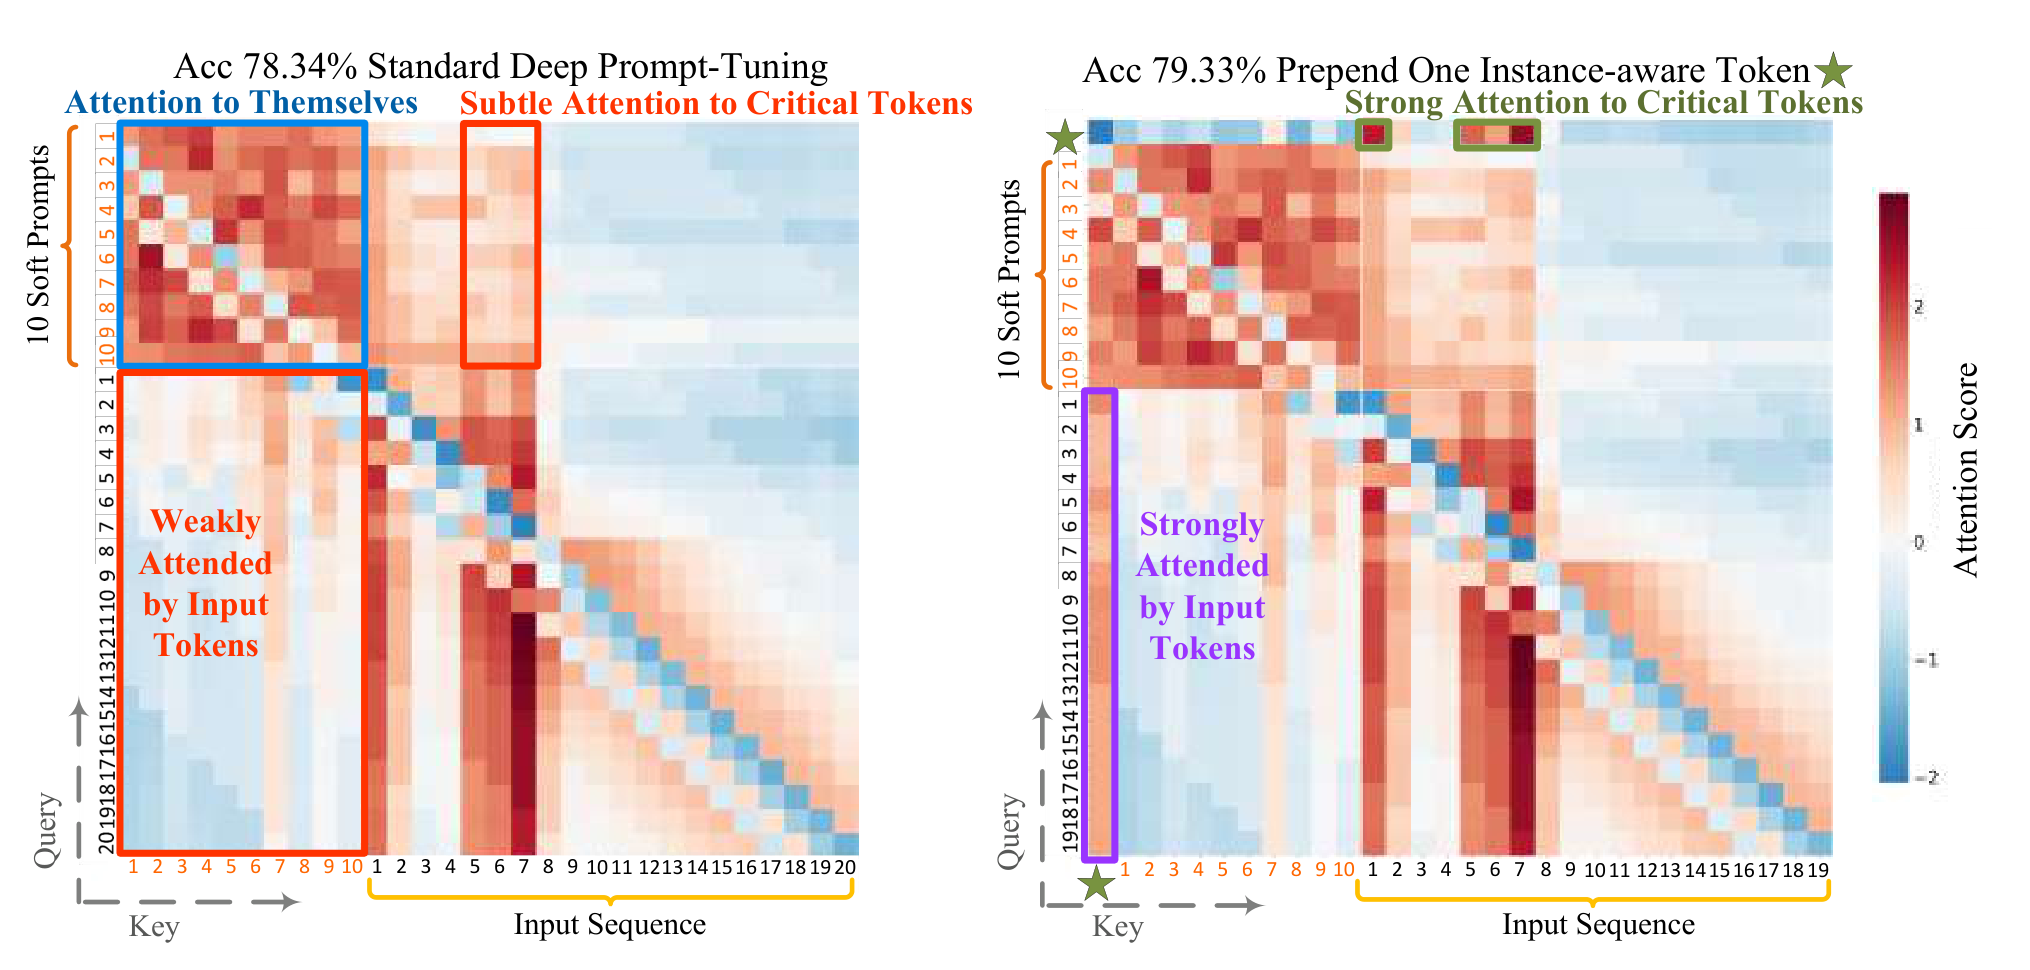
\includegraphics[width=0.74\linewidth]{figures/fig1_attention_softprompt.png}
\src{Attention on T5-Base, RTE (Liu \textit{et al.}, Fig.~1). Red = high attention, blue = low.}
\vspace{2pt}
\begin{columns}[T]
\column{0.47\textwidth}
\small\hl{Left:} 10 soft prompts mostly attend \emph{to each other}; input tokens barely look at them.
\column{0.47\textwidth}
\small\ok{Right:} add \emph{one} instance-aware token $\Rightarrow$ it is strongly attended and points at key tokens. Acc.\ 78.34\% $\to$ 79.33\%.
\end{columns}
\end{frame}

\begin{frame}{Finding II: One Extra Token Helps Without Training}
\begin{columns}[c]
\column{0.56\textwidth}
\centering
\begin{tikzpicture}
\begin{axis}[cleanplot, width=\linewidth, height=5.2cm,
    xlabel={Number of instance-aware tokens added}, ylabel={Accuracy (\%)},
    xtick={0,1,2,3,4,5}, xticklabels={0,1,2,3,4,10},
    ymin=50, ymax=86, legend pos=north east,
    nodes near coords, nodes near coords style={font=\tiny, anchor=south},
    every axis plot/.append style={line width=1pt, mark size=2pt}]
  \addplot[color=navy, mark=*] coordinates {(0,78.3)(1,79.3)(2,78.7)(3,78.3)(4,78.3)(5,74.3)};
  \addplot[color=accent, mark=square*] coordinates {(0,59)(1,63)(2,58)(3,57)(4,54)(5,55)};
  \legend{RTE, COPA}
  \draw[good, dashed, line width=1pt, rounded corners] (axis cs:0.65,52) rectangle (axis cs:1.35,84);
\end{axis}
\end{tikzpicture}
\src{Redrawn from Liu \textit{et al.}, Fig.~2 (T5-Base, test accuracy).}
\column{0.40\textwidth}
\begin{itemize}\setlength\itemsep{6pt}
  \item Take a trained Deep Prompt-Tuning model.
  \item Prepend the \textbf{mean of the input} as an extra token. No retraining.
  \item \ok{1 token}: RTE $+1.0$, COPA $+4.0$.
  \item \hl{More tokens}: accuracy drops.
  \item Lesson: \emph{quality} of guidance matters more than \emph{quantity}.
\end{itemize}
\end{columns}
\end{frame}

\begin{frame}{CaPT Architecture}
\centering
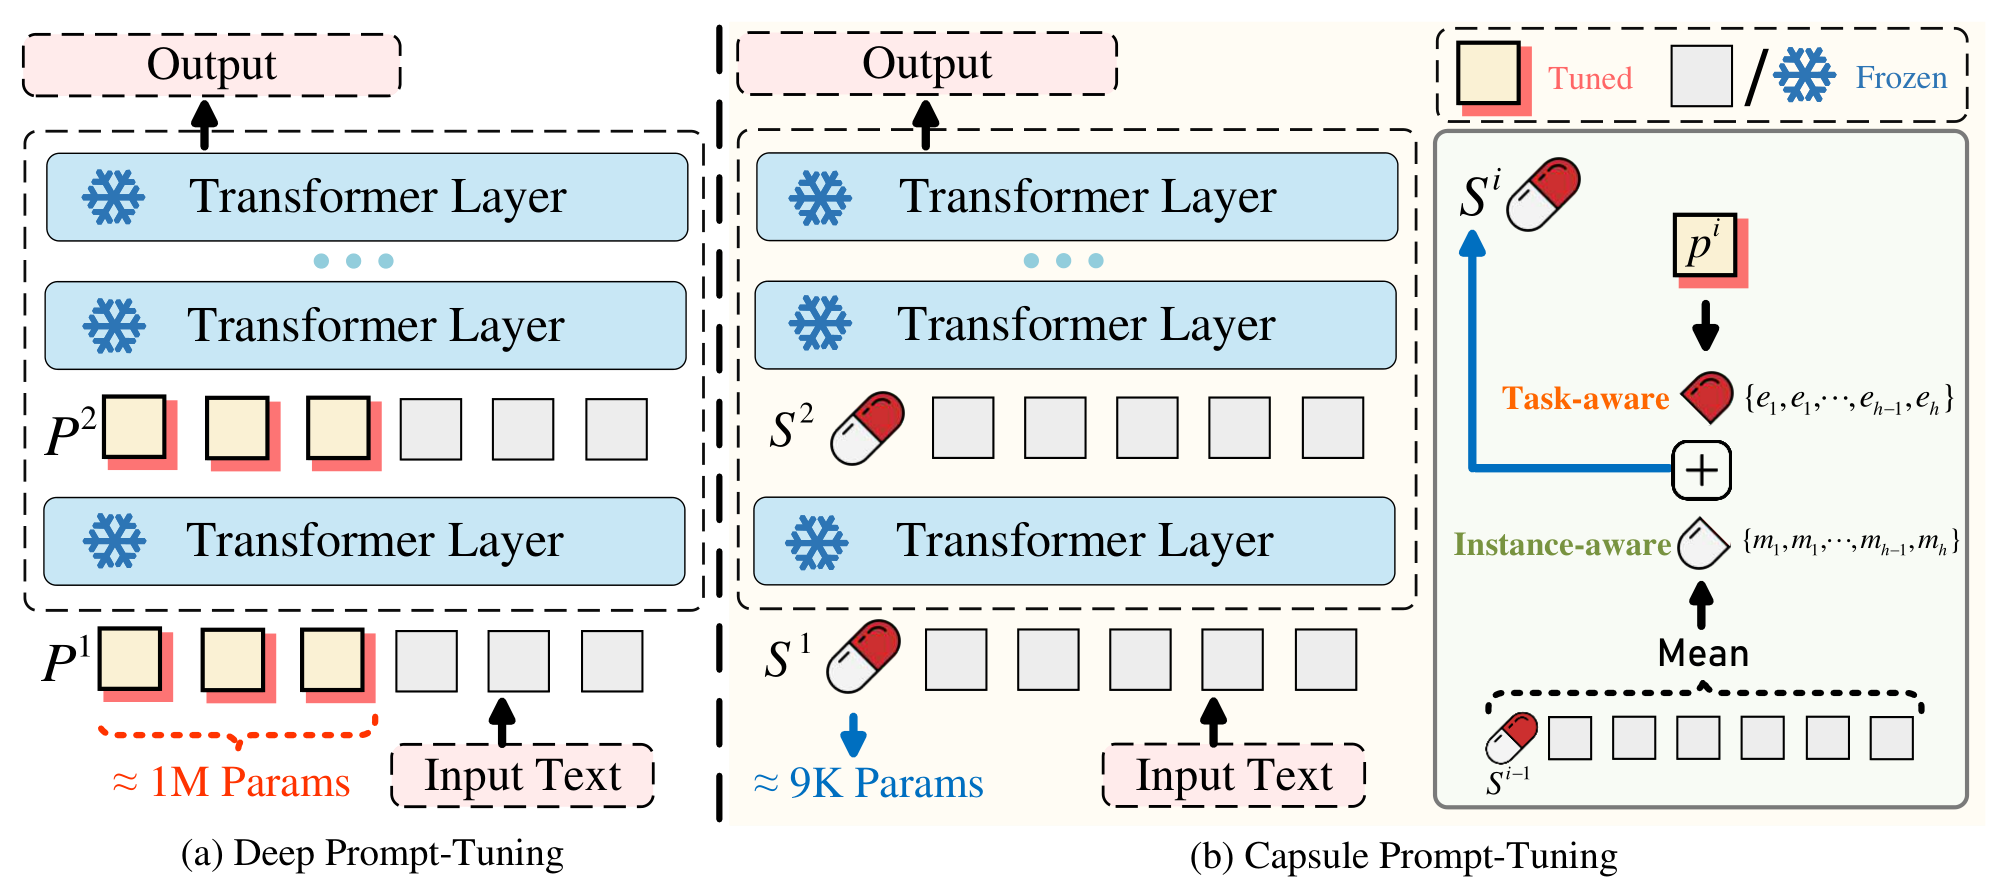
\includegraphics[width=0.82\linewidth]{figures/fig3_framework.png}
\src{Liu \textit{et al.}, Fig.~3. (a) Deep Prompt-Tuning \quad (b) Capsule Prompt-Tuning (CaPT).}
\vspace{4pt}
\begin{columns}[T]
\column{0.45\textwidth}\small\hl{Deep PT:} many trainable prompts per layer $\approx$ \textbf{1M} params.
\column{0.45\textwidth}\small\ok{CaPT:} one capsule per layer $\approx$ \textbf{9K} params (T5-Base).
\end{columns}
\end{frame}

\begin{frame}{How One Capsule is Built (per Layer)}
\centering
\resizebox{\linewidth}{!}{%
\begin{tikzpicture}
  \node[boxgray, text width=2.4cm] (prev) at (0,0) {Previous layer output\\$\underline{S}^{i-1} \oplus H^{i-1}$};
  \node[box, text width=1.6cm] (mean) at (3.0,0) {Mean\\(no params)};
  \node[draw=navy, circle, line width=0.9pt, inner sep=1pt, font=\large] (plus) at (5.4,0) {$+$};
  \node[boxacc, text width=2.2cm] (p) at (5.4,-1.5) {$p^i$: \textbf{1 learnable}\\vector (task)};
  \node[boxgood, text width=1.8cm] (cap) at (7.5,0) {Capsule $S^i$};
  \node[box, text width=2.0cm] (layer) at (10.1,0) {Layer $L_i$\\(frozen)};
  \node[boxgray, text width=1.6cm] (out) at (12.6,0) {$\underline{S}^{i},\ H^{i}$};
  \draw[arr] (prev) -- (mean);
  \draw[arr] (mean) -- node[below, font=\tiny] {input} (plus);
  \draw[arr] (p) -- (plus);
  \draw[arr] (plus) -- (cap);
  \draw[arr] (cap) -- (layer);
  \draw[arr] (layer) -- (out);
  \draw[arr, draw=softgray] (prev.north) -- ++(0,0.55) -| node[pos=0.25, above, font=\tiny, text=softgray]
        {input tokens $H^{i-1}$ go in as usual} (layer.north);
  \draw[arr, draw=softgray] (out.south) -- ++(0,-2.0) -| node[pos=0.25, below, font=\tiny, text=softgray]
        {next layer: $i \to i+1$} (prev.south);
\end{tikzpicture}}

\vspace{8pt}
\begin{columns}[c]
\column{0.48\textwidth}
\small
$S^{1} = p^{1} + \mathrm{Mean}(E)$\\[3pt]
$S^{i} = p^{i} + \mathrm{Mean}\big(\underline{S}^{i-1} \oplus H^{i-1}\big),\ \ i \ge 2$
\column{0.44\textwidth}
\small Only $p^i$ is trained. Length is \textbf{always 1} $\Rightarrow$ nothing to search.
\end{columns}
\end{frame}

\begin{frame}{The ``Attention Anchor'' Effect}
\centering
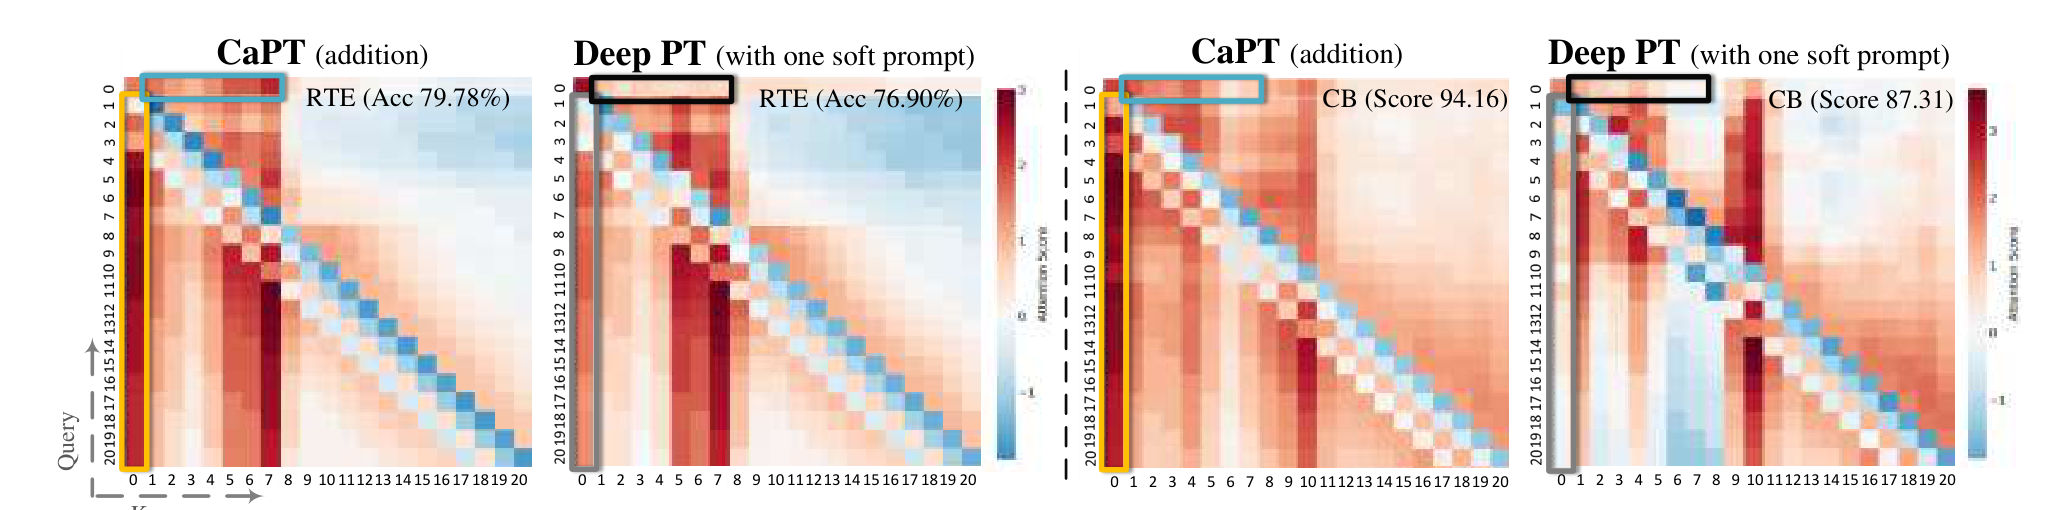
\includegraphics[width=\linewidth]{figures/fig4_attention_anchor.png}
\src{Liu \textit{et al.}, Fig.~4. T5-Base, averaged over all heads and encoder layers (RTE left, CB right).}
\vspace{4pt}
\begin{columns}[T]
\column{0.47\textwidth}
\card[1.3cm]{navy}{Capsule looks at key tokens}{Focuses on structural tokens (e.g.\ ``sentence1:'') -- blue boxes.}
\column{0.47\textwidth}
\card[1.3cm]{good}{All tokens look at the capsule}{Strong column of attention (yellow). CB: 87.31 $\to$ 94.16.}
\end{columns}
\end{frame}

% =====================================================================
\section{Results}

\begin{frame}{Experimental Setup}
\begin{columns}[T]
\column{0.5\textwidth}
\textbf{Datasets} (SuperGLUE)\\[3pt]
\small
\begin{tabular}{@{}ll@{}}
\toprule
\textbf{Task type} & \textbf{Datasets} \\
\midrule
Question answering & BoolQ, MultiRC \\
Natural language inference & CB, RTE \\
Sentence completion & COPA \\
Word sense & WiC \\
\bottomrule
\end{tabular}

\vspace{6pt}
\footnotesize Official validation set used as test set; scores averaged over 3 runs.
\column{0.45\textwidth}
\textbf{Models}\\[3pt]
\begin{tikzpicture}[node distance=2mm]
  \node[box, minimum width=2.6cm] (a) {T5-Base (220M)};
  \node[box, minimum width=2.6cm, below=of a] (b) {T5-Large (770M)};
  \node[boxacc, minimum width=2.6cm, below=of b] (c) {Llama-3.2 (1B)};
  \node[boxacc, minimum width=2.6cm, below=of c] (d) {Qwen-2.5 (1.5B)};
  \node[right=2mm of a, yshift=-3.5mm, font=\scriptsize, text=navy, align=left] {encoder--\\decoder};
  \node[right=2mm of c, yshift=-3.5mm, font=\scriptsize, text=accent, align=left] {decoder-\\only};
\end{tikzpicture}

\vspace{4pt}
\footnotesize \textbf{Baselines:} Fine-Tuning / Linear Head, Prompt-Tuning, P-Tuning v2, XPrompt, SMoP, VFPT, EPT, \dots
\end{columns}
\end{frame}

\begin{frame}{Main Results: Average Score on SuperGLUE}
\begin{columns}[c]
\column{0.64\textwidth}
\centering
\begin{tikzpicture}
\begin{axis}[cleanplot, ybar, width=\linewidth, height=5.6cm,
    bar width=8pt, ymin=50, ymax=92, ylabel={Average score},
    xtick={1,2,3,4}, xticklabels={T5-Base, T5-Large, Llama3.2-1B, Qwen2.5-1.5B},
    enlarge x limits=0.15,
    legend style={at={(0.5,1.02)}, anchor=south, legend columns=-1},
    nodes near coords, nodes near coords style={font=\tiny, rotate=90, anchor=west},
    every node near coord/.append style={/pgf/number format/fixed, /pgf/number format/precision=1}]
  \addplot[fill=gray!45, draw=none] coordinates {(1,72.13)(2,78.16)(3,59.07)(4,58.74)};
  \addplot[fill=navy!65, draw=none] coordinates {(1,76.94)(2,83.79)(3,61.06)(4,61.35)};
  \addplot[fill=accent, draw=none] coordinates {(1,77.51)(2,84.03)(3,67.51)(4,63.17)};
  \legend{Prompt-Tuning, P-Tuning v2, CaPT (ours)}
\end{axis}
\end{tikzpicture}
\src{Data from Liu \textit{et al.}, Table~1.}
\column{0.33\textwidth}
\small
\begin{itemize}\setlength\itemsep{5pt}
  \item \ok{Best} average on all 4 models.
  \item T5-Large: \textbf{84.03} $>$ full fine-tuning (83.60).
  \item T5-Base: 99.6\% of full fine-tuning.
  \item Llama: \textbf{+13.3} points over Linear Head.
  \item Trains only $\le$ \textbf{0.004\%} of parameters.
\end{itemize}
\end{columns}
\end{frame}

\begin{frame}{Main Results: Full Table}
\begin{columns}[c]
\column{0.58\textwidth}
\centering
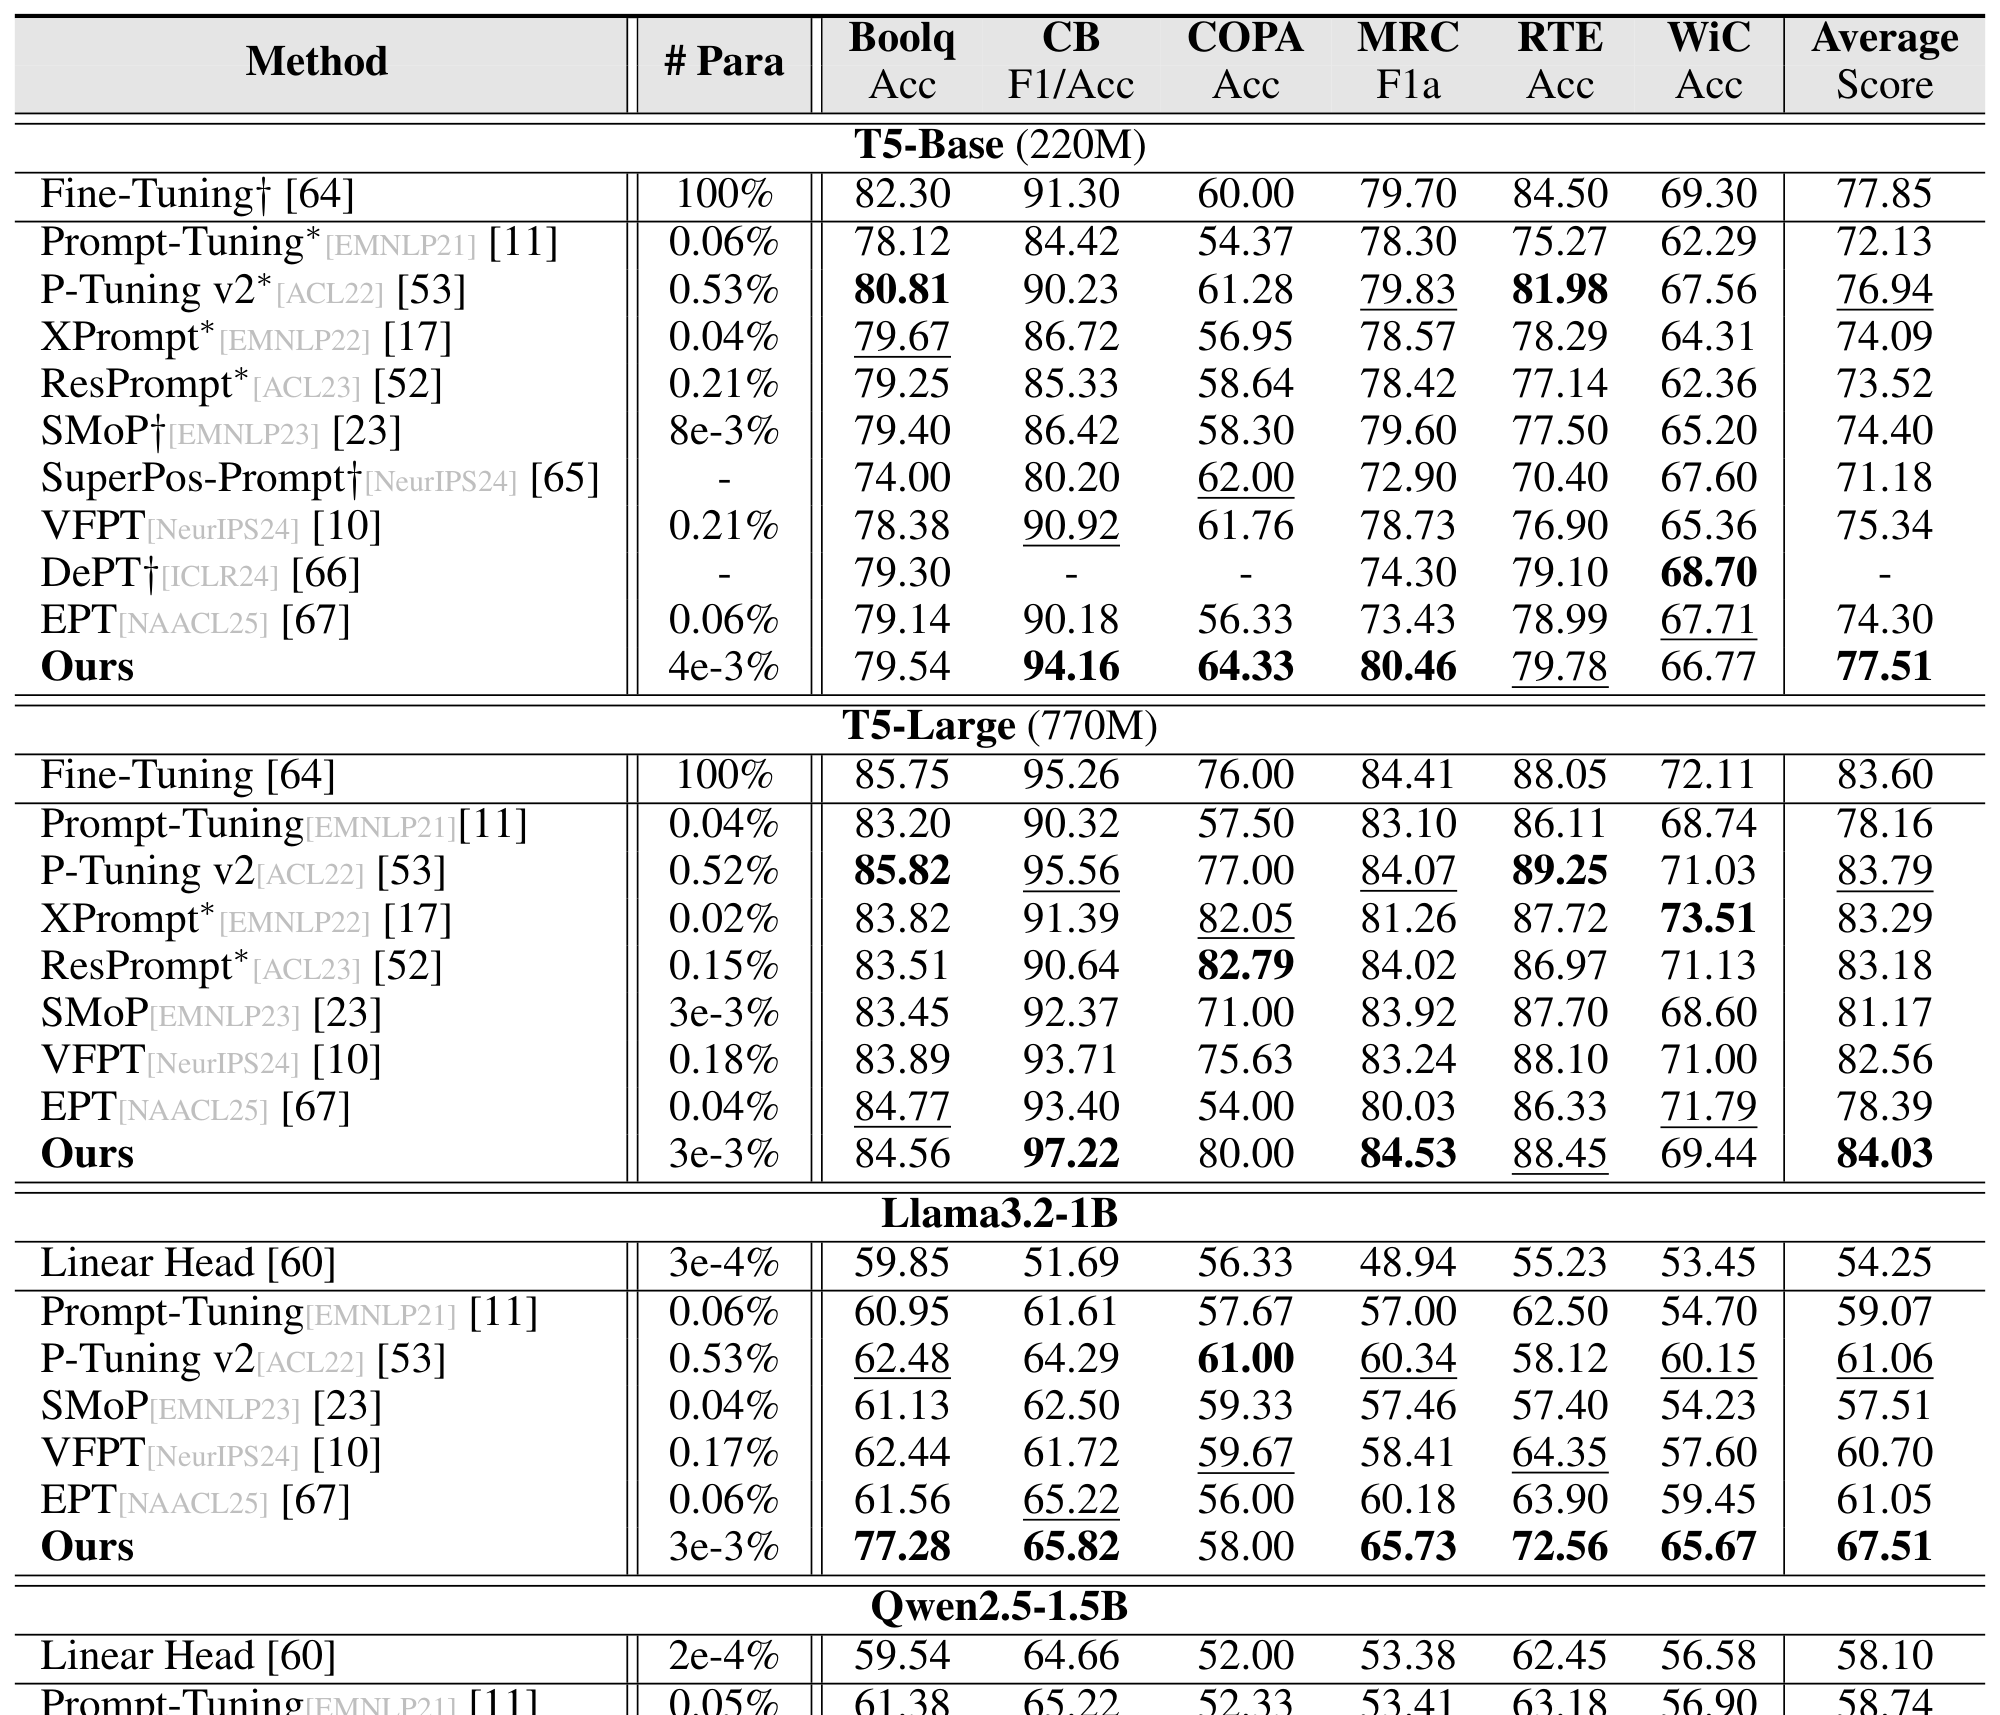
\includegraphics[height=6.1cm]{figures/table1_main_results.png}
\column{0.38\textwidth}
\small
\begin{itemize}\setlength\itemsep{6pt}
  \item \textbf{Bold} = best, \underline{underline} = second best (excluding full fine-tuning).
  \item Gains are \hl{smaller on decoder-only} models (Llama, Qwen) than on T5.
  \item Authors' guess: different pre-training objective and architecture.
\end{itemize}
\src{Liu \textit{et al.}, Table~1.}
\end{columns}
\end{frame}

\begin{frame}{Training Time (T5-Base, incl.\ hyper-parameter search)}
\begin{columns}[c]
\column{0.58\textwidth}
\centering
\begin{tikzpicture}
\begin{axis}[cleanplot, xbar, width=0.9\linewidth, height=5.0cm, bar width=9pt,
    xmin=0, xmax=18, xlabel={Relative training time ($\times$)},
    ytick={1,2,3,4,5}, yticklabels={CaPT (ours), LoPA, M-IDPG, P-Tuning v2, Prompt-Tuning},
    ymajorgrids=false, xmajorgrids, point meta=x,
    nodes near coords={\pgfmathprintnumber[fixed,precision=2]{\pgfplotspointmeta}$\times$},
    nodes near coords style={font=\scriptsize}]
  \addplot[fill=navy!60, draw=none, bar shift=0pt] coordinates {(14.93,2)(12.58,3)(8.37,4)(8.77,5)};
  \addplot[fill=accent, draw=none, bar shift=0pt] coordinates {(1.00,1)};
\end{axis}
\end{tikzpicture}
\column{0.38\textwidth}
\centering\small
\begin{tabular}{@{}lrr@{}}
\toprule
\textbf{Method} & \textbf{Params} & \textbf{Score} \\
\midrule
Prompt-Tuning & 0.06\% & 72.13 \\
P-Tuning v2 & 0.53\% & 76.94 \\
M-IDPG & 0.47\% & 76.96 \\
LoPA & 0.44\% & \textbf{77.98} \\
\textbf{CaPT} & \textbf{0.004\%} & 77.51 \\
\bottomrule
\end{tabular}
\src{Liu \textit{et al.}, Table~2.}
\vspace{4pt}
\raggedright\footnotesize \ok{8--15$\times$ faster} with \ok{100$\times$ fewer} parameters; only LoPA is slightly more accurate.
\end{columns}
\end{frame}

\begin{frame}{Ablation: Capsule Length and Depth}
\begin{columns}[T]
\column{0.48\textwidth}
\centering
\begin{tikzpicture}
\begin{axis}[cleanplot, width=\linewidth, height=4.7cm, title={\footnotesize Length (number of capsules)},
    xtick={1,...,7}, xticklabels={1,2,3,4,5,10,20}, ymin=56, ymax=81, ylabel={Average score},
    legend pos=south west, every axis plot/.append style={line width=1pt, mark size=1.8pt}]
  \addplot[color=navy, mark=*] coordinates {(1,77.51)(2,77.44)(3,73.81)(4,73.85)(5,70.13)(6,70.40)(7,70.35)};
  \addplot[color=accent, mark=square*] coordinates {(1,67.51)(2,67.49)(3,67.04)(4,65.52)(5,65.97)(6,62.13)(7,59.38)};
  \legend{T5-Base, Llama3.2-1B}
\end{axis}
\end{tikzpicture}
\par\centering\small\ok{One capsule is best}; 20 capsules: 67.5 $\to$ 59.4.
\column{0.48\textwidth}
\centering
\begin{tikzpicture}
\begin{axis}[cleanplot, ybar, width=\linewidth, height=4.7cm, title={\footnotesize Depth (which layers get a capsule)},
    bar width=6pt, ymin=55, ymax=81, xtick={1,...,5},
    xticklabels={Input, {1st\\half}, {2nd\\half}, Odd, All}, xticklabel style={align=center},
    enlarge x limits=0.15]
  \addplot[fill=navy!65, draw=none] coordinates {(1,70.55)(2,73.31)(3,73.67)(4,75.28)(5,77.51)};
  \addplot[fill=accent, draw=none] coordinates {(1,59.69)(2,63.75)(3,65.08)(4,65.52)(5,67.51)};
\end{axis}
\end{tikzpicture}
\par\centering\small\ok{All layers best}; spread-out (odd) beats one block.
\end{columns}
\src{Redrawn from Liu \textit{et al.}, Fig.~6.}
\end{frame}

\begin{frame}{Ablation: Ways to Combine Task and Instance Information}
\centering
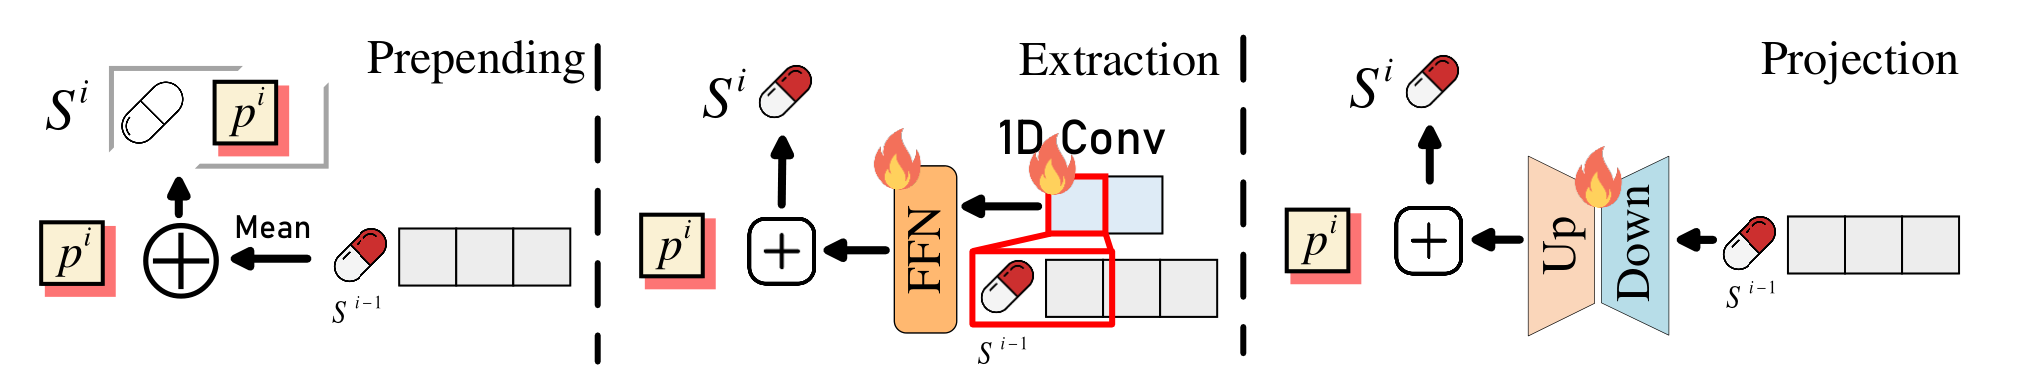
\includegraphics[width=0.9\linewidth]{figures/fig5_variants.png}
\src{Liu \textit{et al.}, Fig.~5. Default design (not shown) = \textbf{Addition}: $S^i = p^i + \mathrm{Mean}(\cdot)$.}
\vspace{6pt}
\begin{columns}[c]
\column{0.42\textwidth}
\centering\small
\begin{tabular}{@{}lrr@{}}
\toprule
\textbf{Variant} & \textbf{Params} & \textbf{Score} \\
\midrule
\textbf{Addition} & \textbf{0.004\%} & 77.51 \\
Prepending & 0.004\% & 77.44 \\
Extraction & 0.03\% & 77.21 \\
Projection & 0.07\% & \textbf{77.64} \\
\bottomrule
\end{tabular}
\column{0.48\textwidth}
\small
\begin{itemize}
  \item All variants work well $\Rightarrow$ the idea is robust.
  \item Addition: nearly the best score with \ok{17.5$\times$ fewer} params than Projection.
\end{itemize}
\end{columns}
\end{frame}

% =====================================================================
\section{Contributions}

\begin{frame}{Contributions of the Paper}
\vspace{4pt}
\begin{columns}[T]
\column{0.47\textwidth}
\card[1.7cm]{navy}{1. New insight}{Task-only soft prompts barely interact with the input; one instance-aware token fixes this.}\\[6pt]
\card[1.7cm]{navy}{2. ``Attention anchor''}{Identified and visualised a two-way attention role for instance-aware tokens.}
\column{0.47\textwidth}
\card[1.7cm]{navy}{3. CaPT method}{One capsule per layer = learnable task vector + input mean. No length search.}\\[6pt]
\card[1.7cm]{good}{4. Strong results}{Best average on 4 LLMs, $\le$0.004\% params, 8--15$\times$ less training time.}
\end{columns}
\end{frame}

% =====================================================================
\section{Limitations}

\begin{frame}{Limitations: Open Research Gaps}
\begin{columns}[T]
\column{0.31\textwidth}
\card[3.9cm]{accent}{Gap 6: Classification only}{
Every task picks a label from a short list.\\[4pt]
\textbf{Missing:} text generation (e.g.\ translation).\\[4pt]
\textbf{Why:} most real LLM use is generation.}
\column{0.31\textwidth}
\card[3.9cm]{accent}{Gap 9: English only}{
All data is English and in-domain.\\[4pt]
\textbf{Missing:} other languages, harder test sets.\\[4pt]
\textbf{Why:} Bangla needs cheap tuning.}
\column{0.31\textwidth}
\card[3.9cm]{accent}{Gap 13: No decoder capsule}{
T5 gets capsules in the \emph{encoder} only.\\[4pt]
\textbf{Missing:} capsules in the decoder.\\[4pt]
\textbf{Why:} in generation, the decoder writes the output.}
\end{columns}
\vspace{4pt}
\src{Other open points: only models $\le$ 1.5B, weaker gains on decoder-only models, attention anchor shown only with pictures.}
\end{frame}

% =====================================================================
\section{Proposal}

\begin{frame}{Our Proposal: Seeing Capsules for Bangla}
\begin{block}{Research question}
Can a \textbf{single image-aware capsule} improve parameter-efficient \textbf{English $\to$ Bangla} multimodal translation?
\end{block}
\vspace{6pt}
\centering
\begin{tikzpicture}[node distance=4mm and 14mm]
  \node[boxacc, text width=4.2cm] (g6) {Gap 6: classification only};
  \node[boxacc, text width=4.2cm, below=of g6] (g9) {Gap 9: English only};
  \node[boxacc, text width=4.2cm, below=of g9] (g13) {Gap 13: no decoder capsule};
  \node[boxgood, text width=6.6cm, right=of g6] (s6) {Generate full Bangla sentences};
  \node[boxgood, text width=6.6cm, right=of g9] (s9) {Bangla target + harder \emph{challenge} test set};
  \node[boxgood, text width=6.6cm, right=of g13] (s13) {Add a capsule to every decoder layer};
  \draw[arr] (g6) -- (s6);
  \draw[arr] (g9) -- (s9);
  \draw[arr] (g13) -- (s13);
  \node[above=1mm of g6, font=\scriptsize\bfseries, text=accent] {Gap};
  \node[above=1mm of s6, font=\scriptsize\bfseries, text=good] {How we address it};
\end{tikzpicture}
\end{frame}

\begin{frame}{Proposed Method}
\centering
\resizebox{\linewidth}{!}{%
\begin{tikzpicture}
  \node[boxgray, text width=1.7cm] (img) at (0,0.9) {Image\\(region)};
  \node[boxgray, text width=1.7cm] (cap) at (0,-0.9) {English\\caption};
  \node[box, text width=1.4cm] (clip) at (2.2,0.9) {CLIP\\(frozen)};
  \node[boxacc, text width=1.5cm] (lin) at (4.0,0.9) {Linear\\(trainable)\\[1pt]{\tiny $\to$ image token}};
  \node[box, text width=2.2cm, minimum height=2.6cm] (enc) at (7.3,0) {\textbf{mT5 Encoder}\\(frozen)\\[4pt]+ capsule $c_{\text{enc}}$};
  \node[box, text width=2.2cm, minimum height=2.6cm] (dec) at (10.1,0) {\textbf{mT5 Decoder}\\(frozen)\\[4pt]+ capsule $c_{\text{dec}}$};
  \node[boxgood, text width=1.8cm] (out) at (12.8,0) {Bangla\\sentence};
  \draw[arr] (img) -- (clip);
  \draw[arr] (clip) -- (lin);
  \draw[arr] (lin.east) -- (enc.west |- lin.east);
  \draw[arr] (cap.east) -- node[above, font=\tiny] {text tokens} (enc.west |- cap.east);
  \draw[arr] (enc) -- (dec);
  \draw[arr] (dec) -- (out);
  \node[font=\scriptsize, text=accent] at (7.3,-1.75) {$c_{\text{enc}} = p_{\text{enc}} + \mathrm{mean}(\text{image} + \text{text})$};
  \node[font=\scriptsize, text=accent] at (10.4,-2.2) {$c_{\text{dec}} = p_{\text{dec}} + \mathrm{mean}(\text{encoder output})$};
\end{tikzpicture}}

\vspace{8pt}
\begin{columns}[T]
\column{0.31\textwidth}\card[1.7cm]{navy}{Image-aware capsule}{The image is one more token, so the capsule sees it.}
\column{0.31\textwidth}\card[1.7cm]{navy}{Decoder capsule}{Brings text + image to the part that writes Bangla.}
\column{0.31\textwidth}\card[1.7cm]{navy}{Still tiny}{Masked mean (no padding); mT5 stays frozen.}
\end{columns}
\end{frame}

\begin{frame}{Data, Experiments and Metrics}
\begin{columns}[T]
\column{0.36\textwidth}
\textbf{Dataset:} Bengali Visual Genome\\
\footnotesize English caption + Bangla translation + image region.\\
Has a \textbf{challenge test set} with ambiguous English words.

\vspace{8pt}
\normalsize\textbf{Model:} mT5-Base (frozen)\\
\footnotesize Backup: BanglaT5.

\vspace{8pt}
\normalsize\textbf{Metrics}\\
\footnotesize chrF++ (main), BLEU, trainable params, training time. 3 seeds, mean $\pm$ std.
\column{0.6\textwidth}
\centering\footnotesize
\renewcommand{\arraystretch}{1.15}
\begin{tabular}{@{}clc@{}}
\toprule
\textbf{\#} & \textbf{Setting} & \textbf{Answers} \\
\midrule
1 & Frozen mT5 (no training) & lower bound \\
2 & Prompt-Tuning baseline & baseline \\
3 & CaPT, text only, encoder only & Gap 6 \\
4 & + decoder capsule & Gap 13 \\
5 & + image token & image helps? \\
6 & Exp.\ 5 with mismatched images & image really used? \\
7 & Exps.\ 3--6 on challenge set & Gap 9 \\
\bottomrule
\end{tabular}
\end{columns}
\end{frame}

\begin{frame}{Work Plan (4 Weeks)}
\centering
\begin{tikzpicture}[x=2.2cm, y=0.85cm]
  \foreach \wk in {1,...,4} {
    \node[font=\footnotesize\bfseries, text=navy] at (\wk+0.5,0.6) {Week \wk};
    \draw[gray!30] (\wk,0.3) -- (\wk,-4.3);
  }
  \draw[gray!30] (5,0.3) -- (5,-4.3);
  \foreach \yy/\st/\txt/\col in {
      -0.5/1/{Setup, data, CLIP features, Exp.\ 1--2}/navy,
      -1.5/2/{Masked mean, decoder capsule (Exp.\ 3--4)}/navy,
      -2.5/3/{Image token (Exp.\ 5--6)}/good,
      -3.5/4/{Challenge set (Exp.\ 7), report}/accent} {
    \node[draw=\col, fill=\col!15, rounded corners=2pt, minimum height=0.6cm,
          minimum width=2.1cm, anchor=west] at (\st+0.02,\yy) {};
    \node[anchor=east, font=\footnotesize, align=right, text width=4.4cm] at (0.9,\yy) {\txt};
  }
\end{tikzpicture}

\vspace{6pt}
\small \textbf{Minimum result:} Exps.\ 1--4 alone (CaPT for Bangla generation with a decoder capsule) form a complete study.
\quad \textbf{Compute:} free Colab / Kaggle GPUs (16 GB).
\end{frame}

% =====================================================================
\section{Conclusion}

\begin{frame}{Conclusion}
\begin{columns}[c]
\column{0.55\textwidth}
\begin{itemize}\setlength\itemsep{6pt}
  \item Soft prompts that know only the \emph{task} miss the \emph{input}.
  \item CaPT: \textbf{one capsule} = learnable task vector + mean of the input.
  \item It acts as an \textbf{attention anchor} and gives the best average score with $\le$0.004\% params and no length search.
  \item Open gaps: only \hl{classification}, only \hl{English}, \hl{no decoder capsule}.
  \item We propose to close them with image-aware capsules for \ok{English $\to$ Bangla} translation.
\end{itemize}
\column{0.4\textwidth}
\begin{exampleblock}{Take-home message}
For prompt tuning, \textbf{one well-informed vector} can beat many uninformed ones.
\end{exampleblock}
\end{columns}
\end{frame}

\begin{frame}{References}
\scriptsize
\begin{enumerate}\setlength\itemsep{3pt}
  \item Y.~Liu \textit{et al.} All You Need is One: Capsule Prompt Tuning with a Single Vector. \textit{NeurIPS}, 2025.
  \item B.~Lester, R.~Al-Rfou, N.~Constant. The Power of Scale for Parameter-Efficient Prompt Tuning. \textit{EMNLP}, 2021.
  \item X.~Liu \textit{et al.} P-Tuning v2: Prompt Tuning Can Be Comparable to Fine-tuning Across Scales and Tasks. \textit{ACL}, 2022.
  \item E.~J.~Hu \textit{et al.} LoRA: Low-Rank Adaptation of Large Language Models. \textit{ICLR}, 2022.
  \item N.~Houlsby \textit{et al.} Parameter-Efficient Transfer Learning for NLP. \textit{ICML}, 2019.
  \item C.~Raffel \textit{et al.} Exploring the Limits of Transfer Learning with a Unified Text-to-Text Transformer. \textit{JMLR}, 2020.
  \item A.~Wang \textit{et al.} SuperGLUE: A Stickier Benchmark for General-Purpose Language Understanding Systems. \textit{NeurIPS}, 2019.
  \item G.~Xiao \textit{et al.} Efficient Streaming Language Models with Attention Sinks. \textit{ICLR}, 2024.
\end{enumerate}
\end{frame}

\begin{frame}[plain]
\begin{tikzpicture}[remember picture,overlay]
  \fill[navy] (current page.south west) rectangle (current page.north east);
  \fill[accent] ([yshift=-0.6cm]current page.west) rectangle ([yshift=-0.68cm]current page.east);
  \node[text=white, font=\Huge\bfseries] at ([yshift=0.3cm]current page.center) {Thank You!};
  \node[text=white!80!navy, font=\large] at ([yshift=-1.3cm]current page.center) {Questions?};
\end{tikzpicture}
\end{frame}

\end{document}
